
\subsection{Proprioception}

\begin{frame}{Estimation de l'odométrie (1/3) -- Modèle géométrique}
    \begin{columns}
        \begin{column}{0.45\linewidth}
            Humanoïdes $\Rightarrow$ déplacement \og sous actué \fg\\
            \vspace{1.0em}
            \begin{block}{Modèle géométrique direct}
                espace articulaire (moteurs) $\longmapsto$ espace cartésien (monde 3D)
            \end{block}
            \vspace{1.0em}
            Hypothèses :
            \begin{itemize}
                \item Pas de glissement
                \item Toujours un pied au sol
                \item Pas de double support
                \item Pied de support non posé à plat
            \end{itemize}
        \end{column}
        \begin{column}{0.55\linewidth}
            \centering
            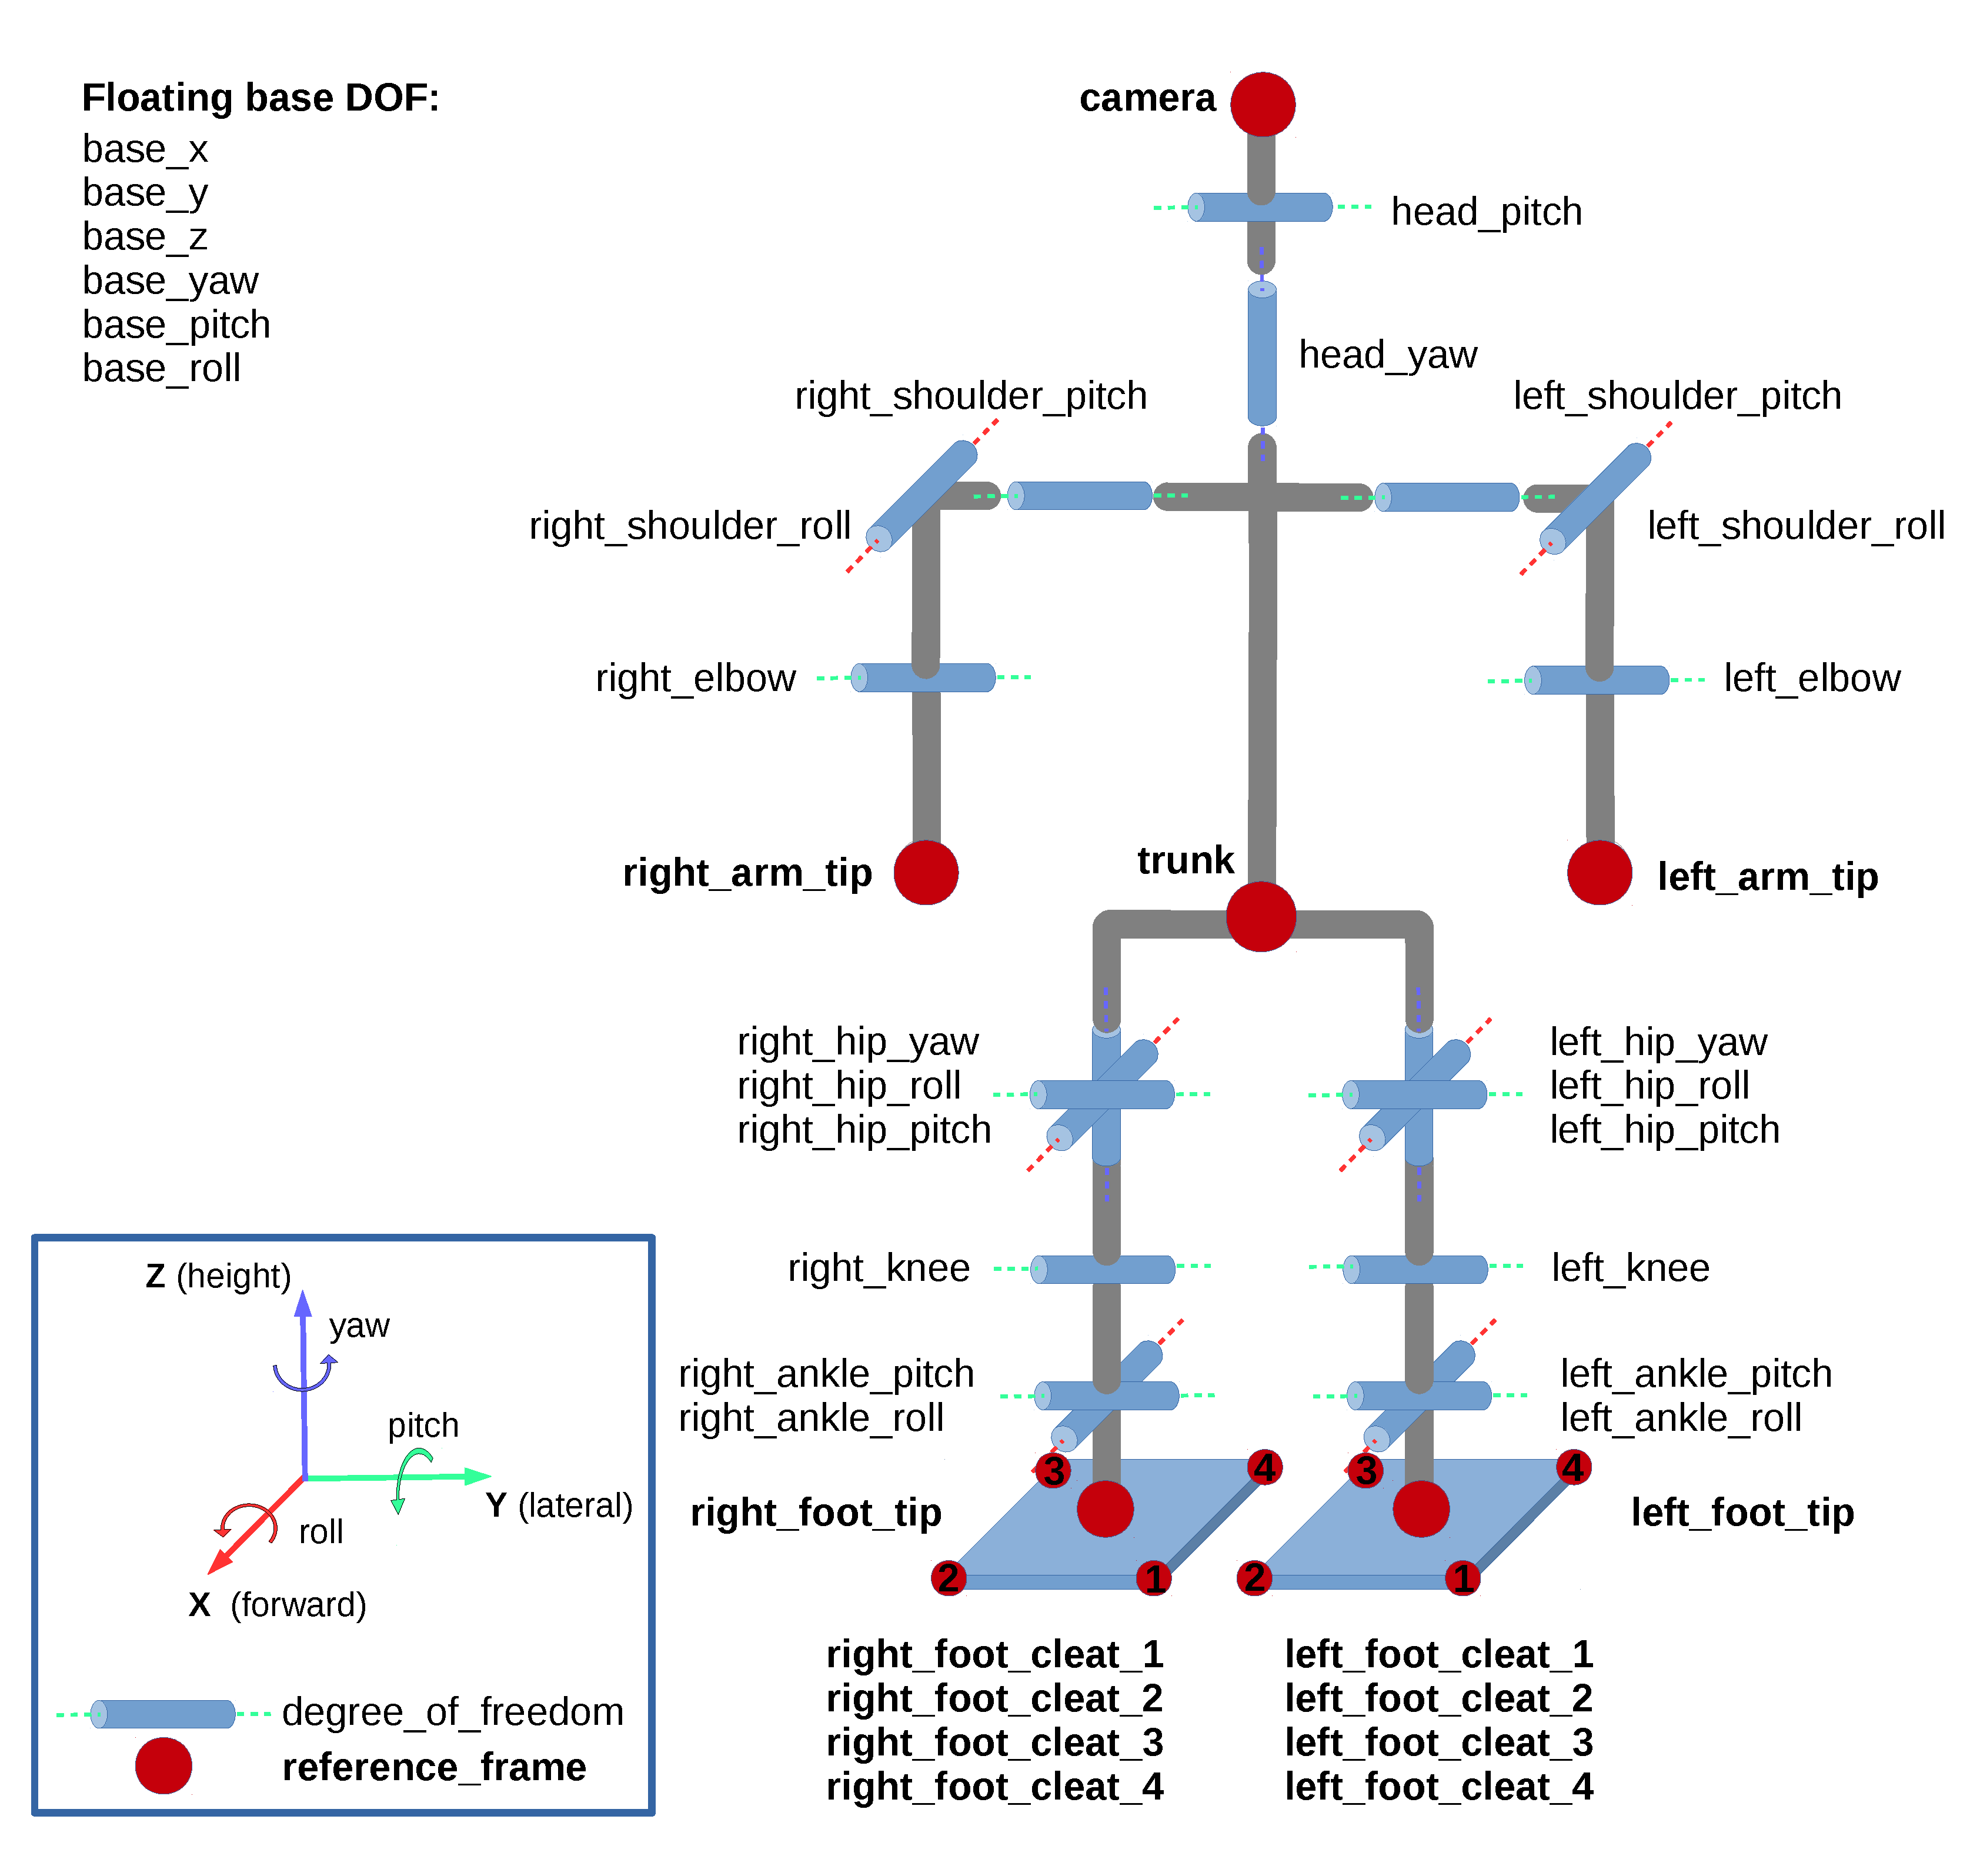
\includegraphics[type=pdf,ext=.pdf,read=.pdf,width=1.0\linewidth]{../schema/humanoid}
        \end{column}
    \end{columns}
\end{frame}

\begin{frame}{Estimation de l'odométrie (2/3) -- Proprioception}
    \begin{columns}
        \begin{column}{0.5\linewidth}
            Capteurs :
            \begin{itemize}
                \item Estimation du pied de support
                \item Encodeurs $\Rightarrow$ angles articulations
                \item Centrale inertielle (IMU) :
                    \begin{itemize}
                        \item accéléromètres, gyromètres
                        \item filtrage de Mahony
                        \item inclinaison du buste
                    \end{itemize}
                \item Intégration des gyromètres $\Rightarrow$ azimut du buste
            \end{itemize}
        \end{column}
        \begin{column}{0.5\linewidth}
            \centering
            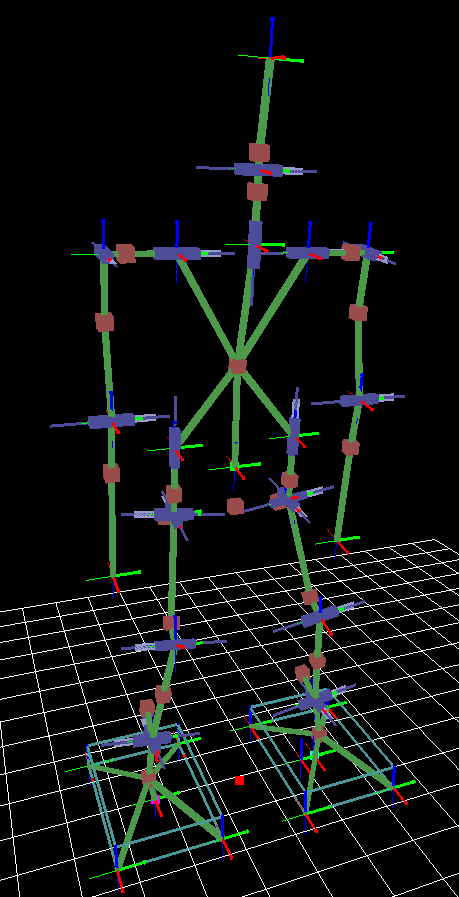
\includegraphics[height=0.85\textheight]{../media/model_gui1.png}
        \end{column}
    \end{columns}
\end{frame}

\begin{frame}{Estimation de l'odométrie (3/3) -- Intégration}
    \begin{columns}
        \begin{column}{0.5\linewidth}
            Odométrie proprioceptive :
            \begin{itemize}
                \item Capteurs $\Rightarrow$ état géométrique
                \item Au changement de pied de support :
                    \begin{itemize}
                        \item Calcul de la pose du deuxième pied
                        \item Changement et conversion du modèle géométrique (autre pied)
                    \end{itemize}
            \end{itemize}
            \vspace{1.0em}
            Odométrie prédictive :
            \begin{itemize}
                \item Ordres de déplacement $\Rightarrow$ générateur de marche $\Rightarrow$
                    positions articulaires désirées
                \item Pied à plat sur le sol
                \item Pied de support imposé par la marche
            \end{itemize}
        \end{column}
        \begin{column}{0.5\linewidth}
            \centering
            \movie[
                autostart,
                width=\linewidth, 
                height=0.76\linewidth,
                poster,
                loop
            ]{}{../video/walk.ogv}
        \end{column}
    \end{columns}
\end{frame}

